\section{Development and Implementation}
\subsection{Electrical}
\subsection{Motors}
The custom servo motors posed a very interesting challenge when it came to size and component density. On a board that had to fit in an 18mmx36mm space a micro controller, magnetic encoder, voltage regulator, 2 connectors, a motor driver and a motor along with all supporting circuitry. This along with some simple oversights meant the board went through 2 major revisions and 1 minor revision. 

\begin{figure}[H]
       \centering
       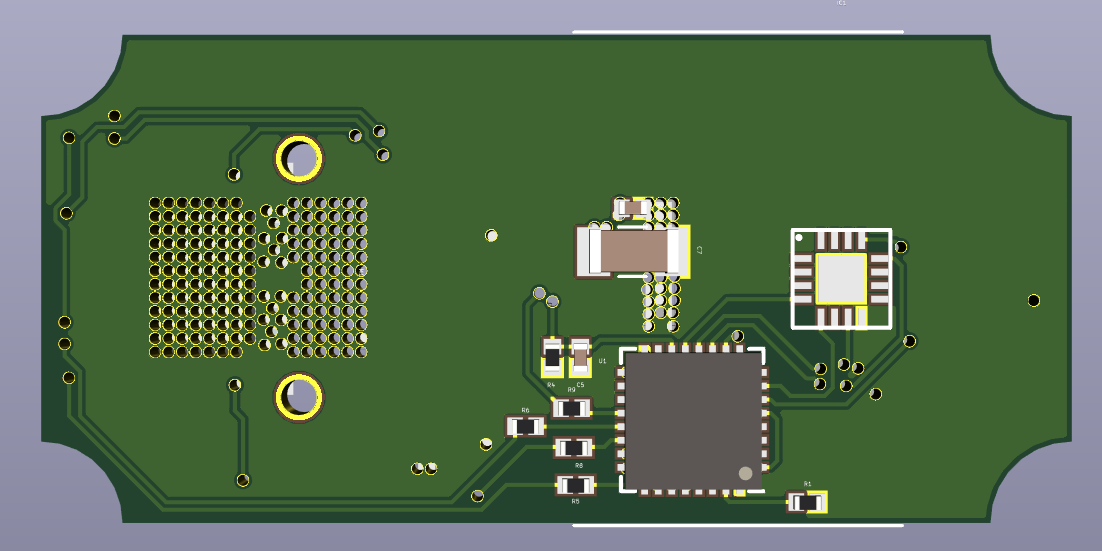
\includegraphics[width=0.6\textwidth]{figures/MotorControllerBottom.png}
       \caption{Motor controller PCB bottom}
       \label{fig:my_label}
   \end{figure}
   \begin{figure}[H]
       \centering
       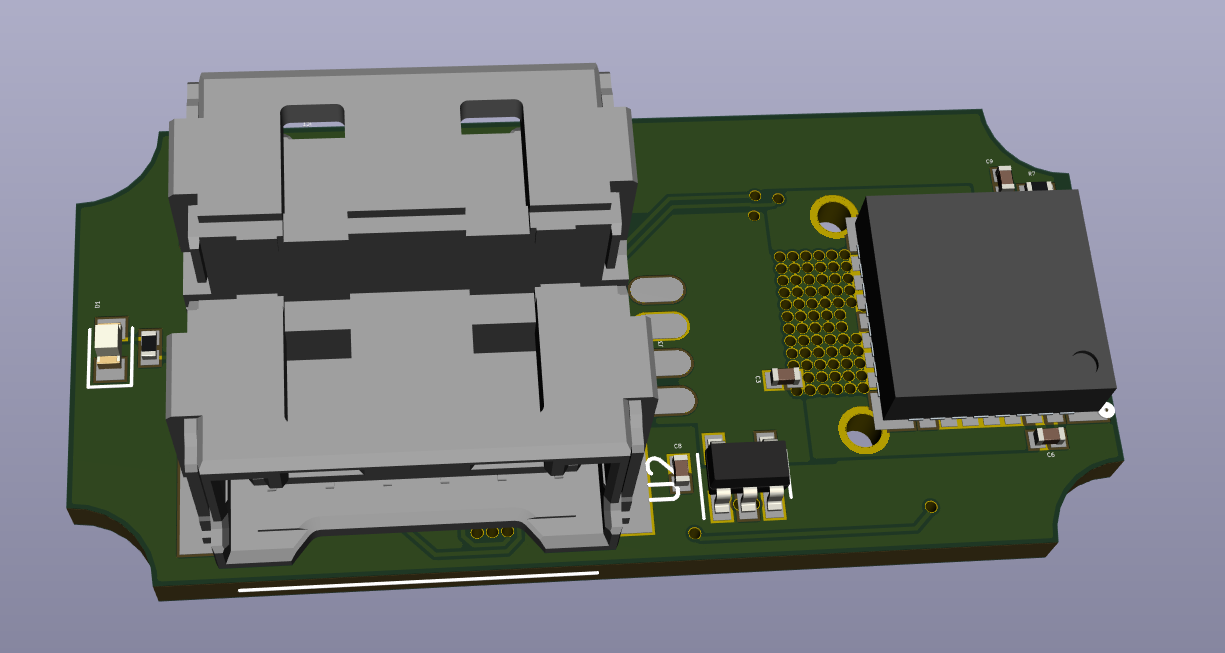
\includegraphics[width=0.6\textwidth]{figures/MotorControllerTop.png}
       \caption{Motor controller PCB top}
       \label{fig:my_label}
   \end{figure}
The boards were designed to be assembled directly into the motor connected directly by the motor pins, aligning the encoder above the magnet connected directly to the output shaft of the motor. The programming header was designed as a series of pads that can be used in combination with a pogo pin programming jig, meaning that the firmware can be updated quickly and easily. 
\subsection{Motherboard}
The mother board was developed to be a stand alone micro controller using the STM32H743iit6 micro controller running at 400 MHz. Broken out from this micro controller were all 6 SPI channels, 12 GPIO pins, UART, USB HS and a programming header. In order to limit the number of traces interfering with the High power  coming from the battery, 3.3v and the Ground Plane a 4 layer board was chosen despite the increased cost of production. This meant that all the signal traces could be run internally allowing for a continuous trace running around the periphery of the board connecting all of the connectors to the 8.4v supply coming in from the battery.
\begin{figure}[H]
       \centering
       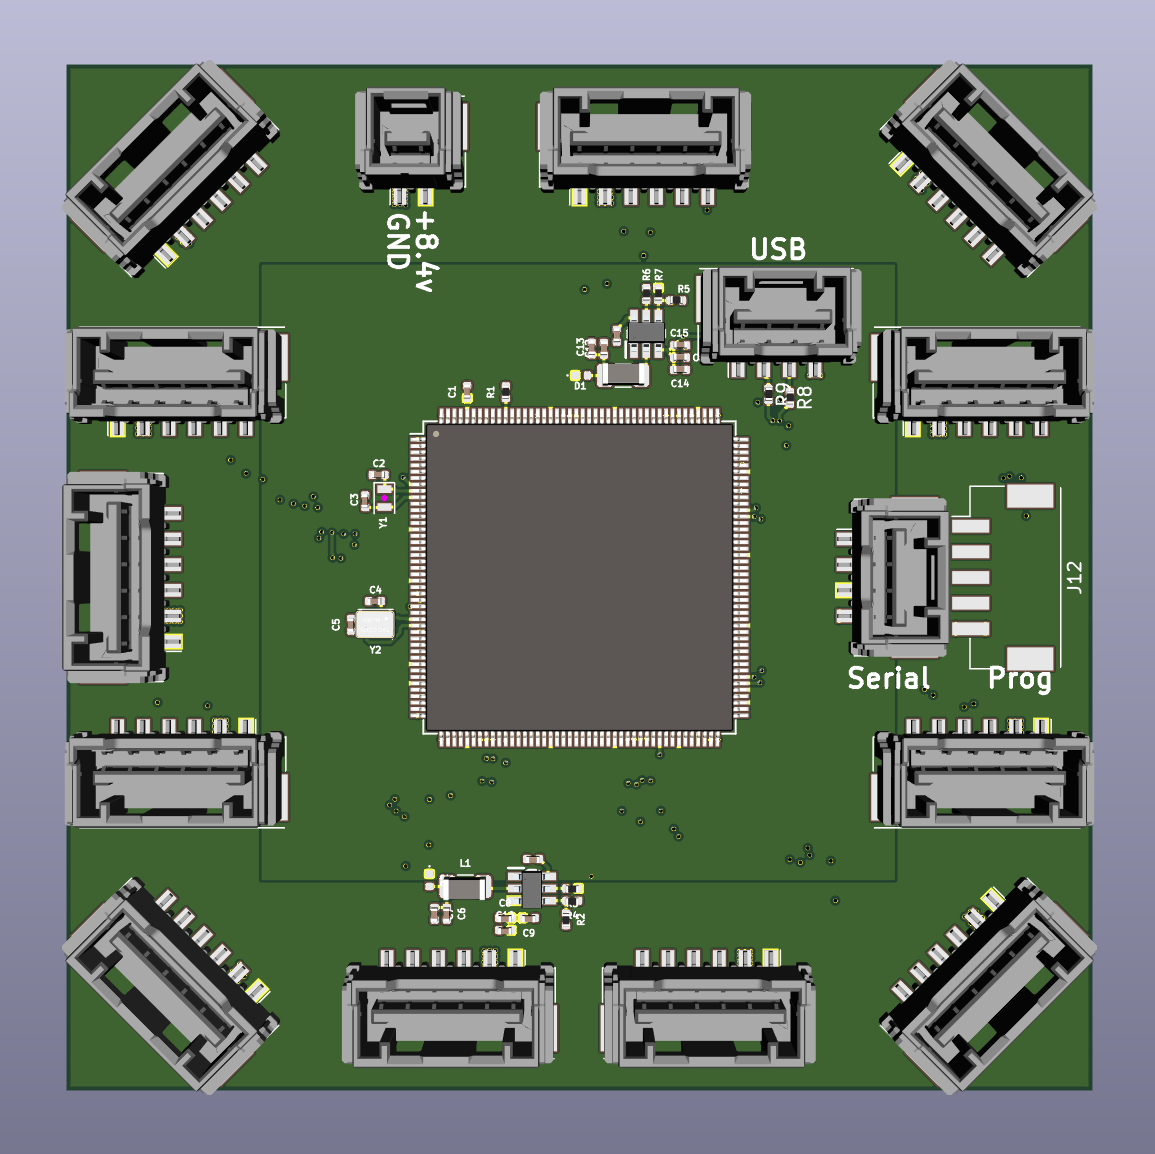
\includegraphics[width=0.6\textwidth]{figures/Motherboard.png}
       \caption{Motherboard}
       \label{fig:my_label}
   \end{figure}
To ensure reliability at higher clock speeds both a 32.768 kHz crystal oscillator and a 32MHz crystal oscillator were used. While developing the firmware for the motherboard the the clock speed was reduced from 400MHZ to 384 MHz in order to optimize the speed at which the SPI could be run as a clock divisible by 24MHz was requires to take full advantage of the SPI communication with the micro controllers on the motors. In order to have a reliable and stable 3.3v rail for the micro controller, 2 switch mode buck converter power supplies were used in order to stop regulate the 5v supply from USB and the 8.4v supply from the battery pack. This allows the board to be developed on and tested using only power from the USB connection and does not require the battery be connected. 
  
   The motherboard was designed and went through one minor revision to remedy an error in the switch mode power supply circuit as well as to change from USB FS to USB HS allowing for a much faster data  through put at up to 48Mb/s
\subsection{IMU}

\subsection{Foot Sensors}